\documentclass[../main.tex]{subfiles}

\begin{document}

\subsubsection*{Methodology}
    Laser light can not only be characterized through its wavelengths, but also through the light modes in the resonator. The goal of this section is to make some of these modes next to the dominant gaussian mode visble. Again, the setup in figure \ref{fig:4-Aufbau} is used. A thin hair is brought into the laser beam, once in a vertical position and once in a horizontal one. The beam is then disrupted along the intersection with the hair line and modes with minimal intensity along the hair line are preferred, instead of the gaussian mode.

\subsubsection*{Data analysis}
    We observe two modes in the resonator of the HeNe laser. They are displayed in figure \ref{fig:TEM_0_1} and \ref{fig:TEM_1_0}.
    \begin{figure}[H]
        \centering
        \begin{subfigure}[b]{0.4\textwidth}
            \centering
            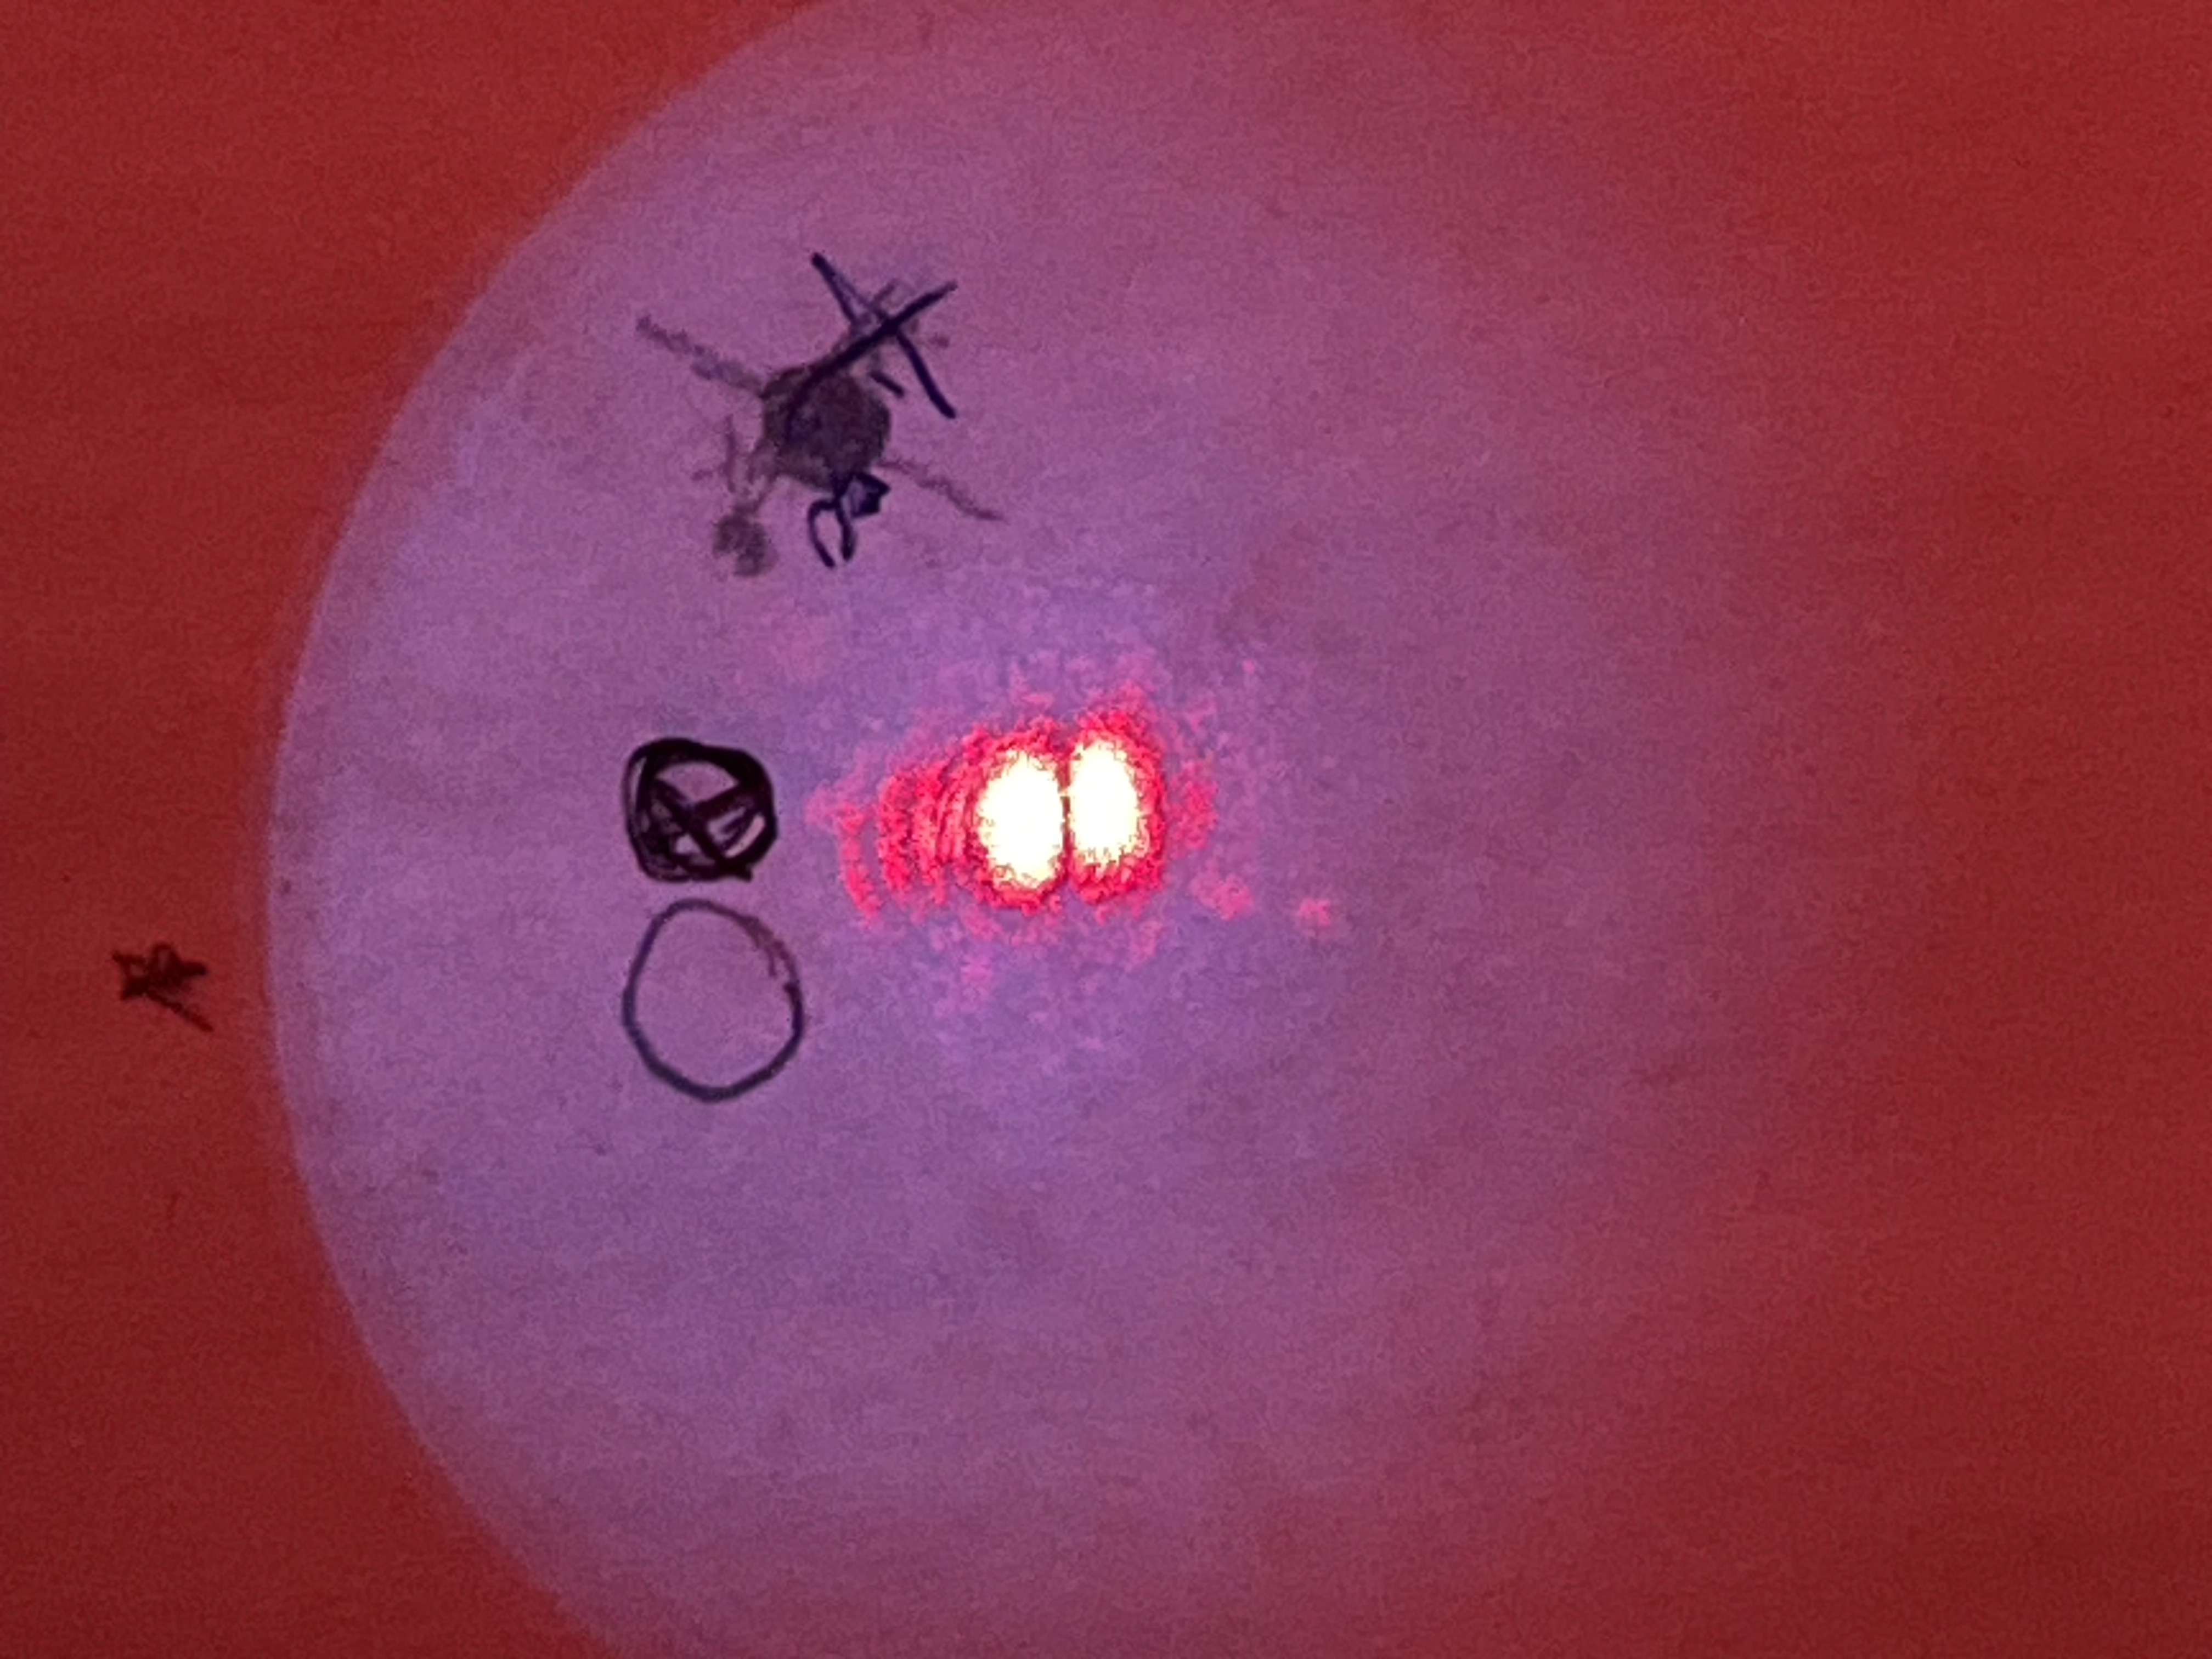
\includegraphics[angle=0,width=\textwidth]{Bilddateien/6/IMG_3497.jpeg}
            \caption{$\text{TEM}_{0,1}$}
            \label{fig:TEM_0_1}
        \end{subfigure}
        \begin{subfigure}[b]{0.4\textwidth}
            \centering
            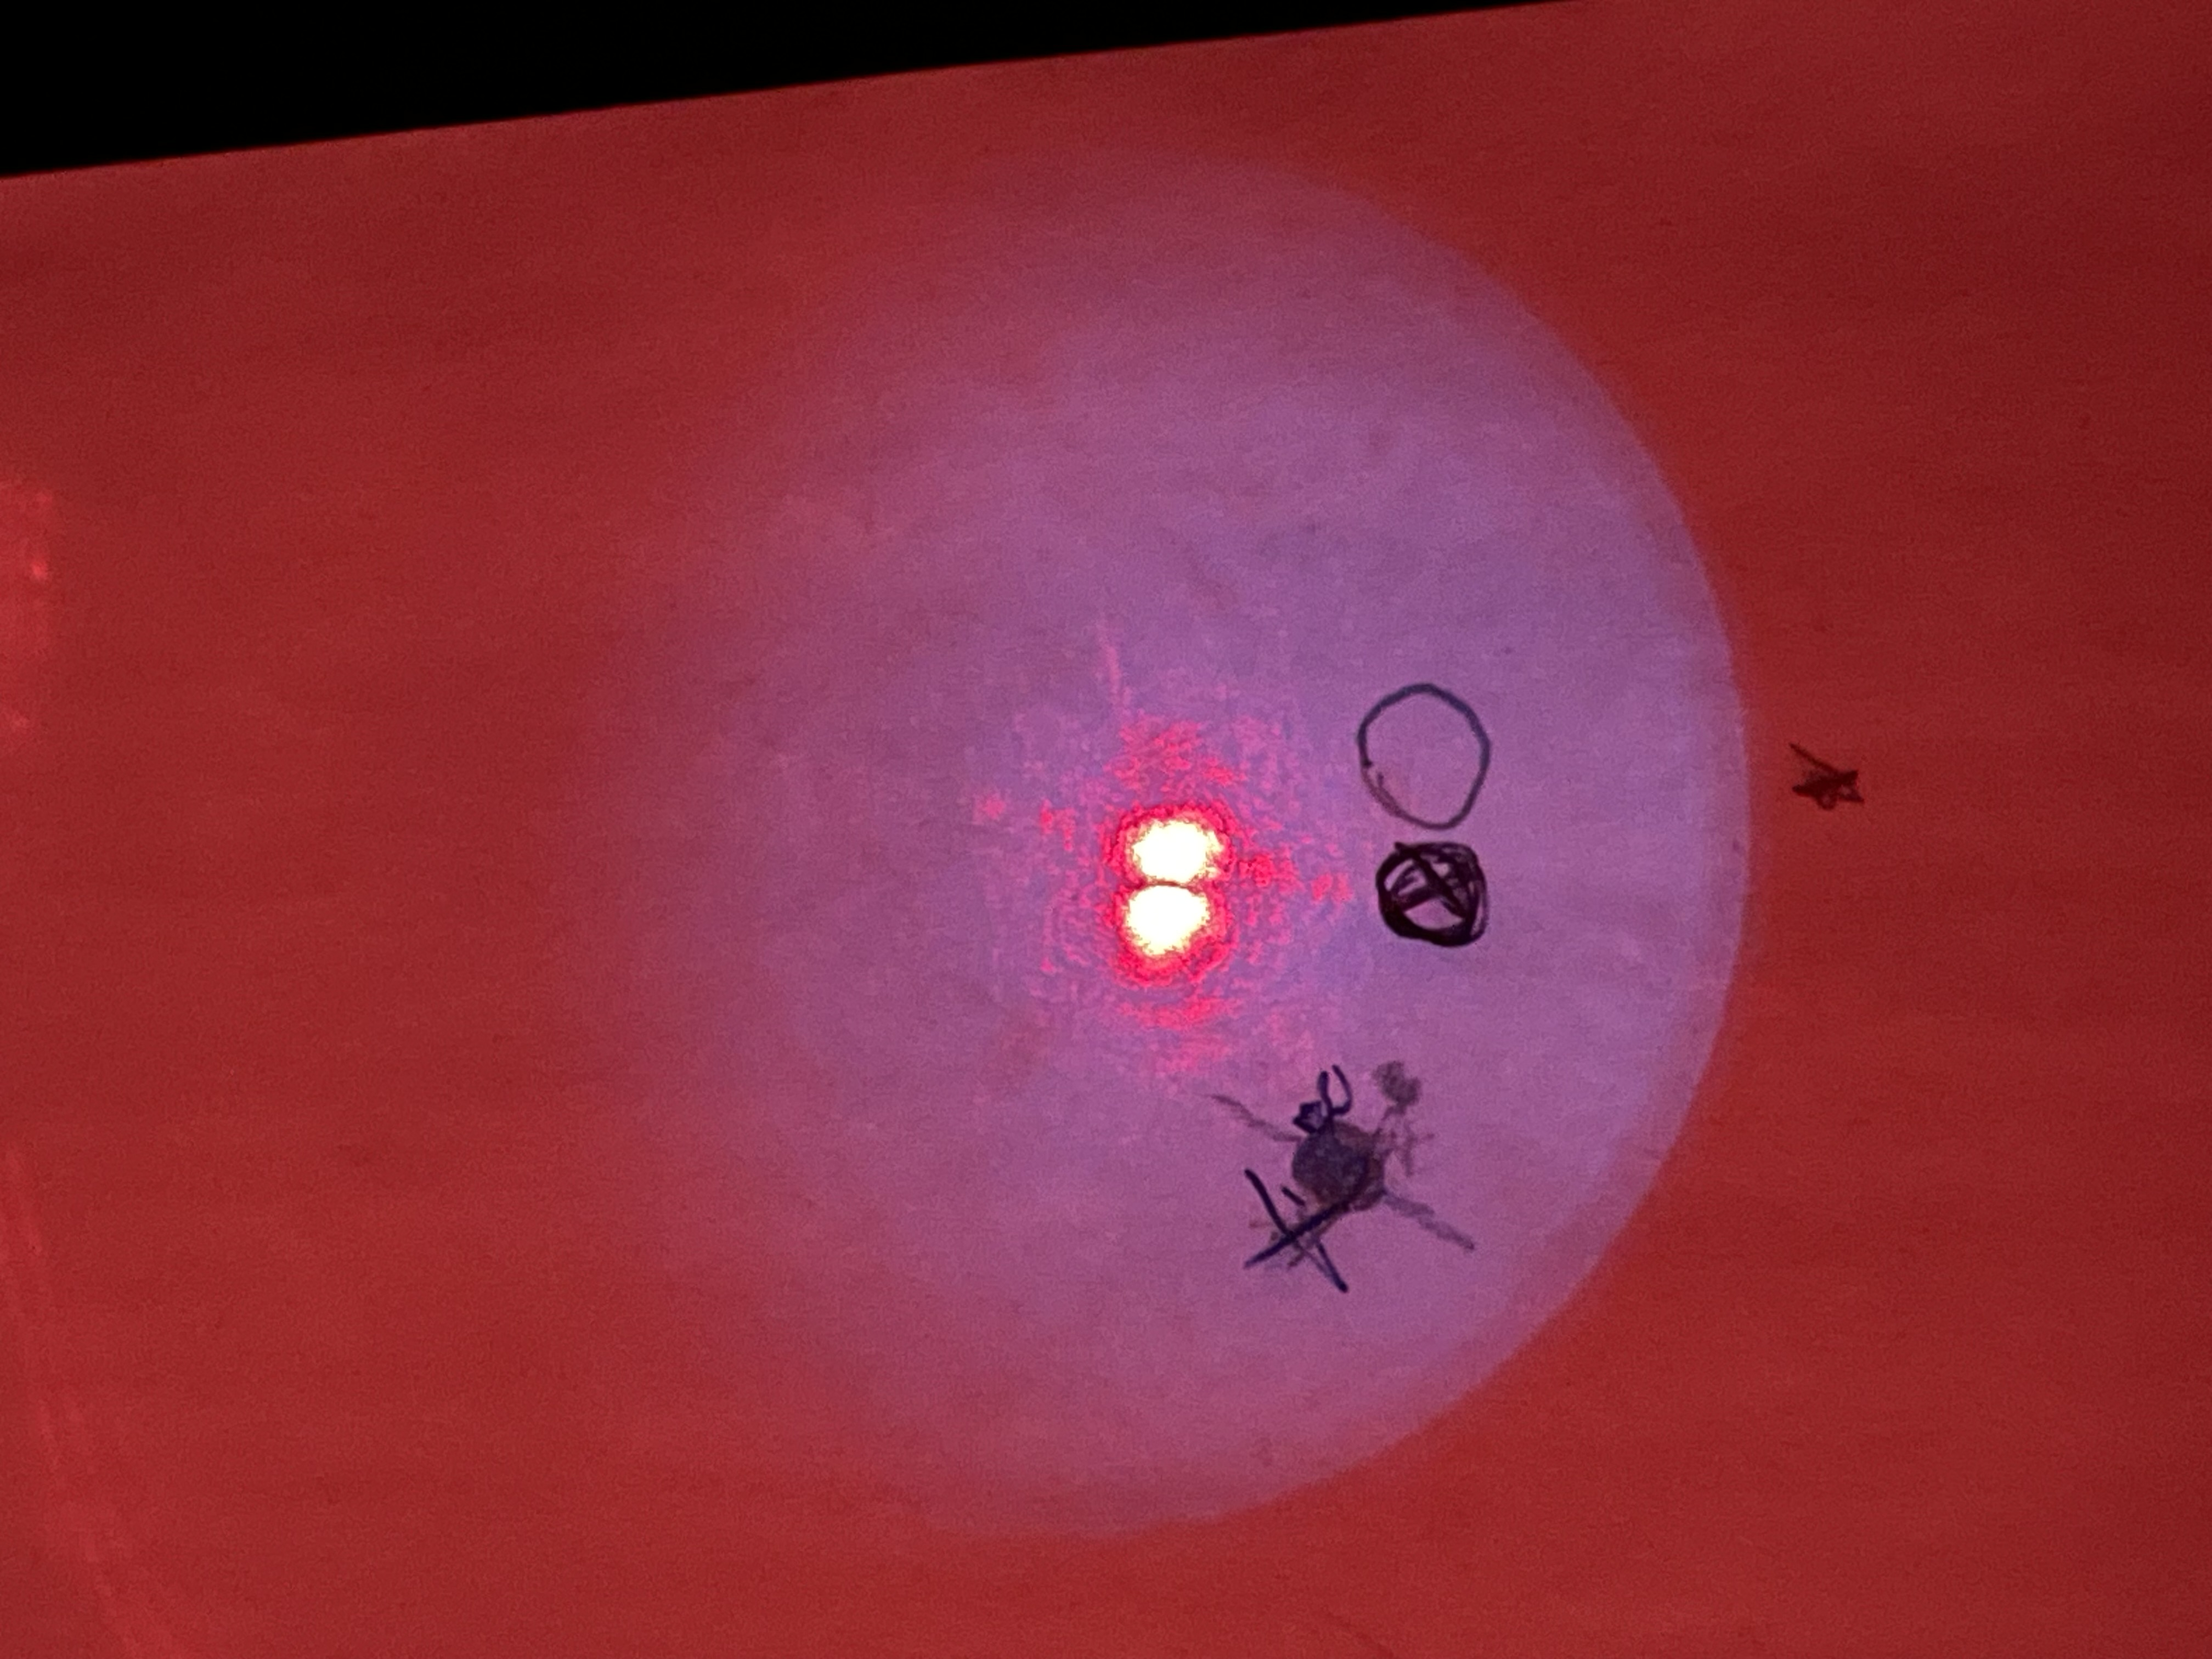
\includegraphics[angle=180,width=\textwidth]{Bilddateien/6/IMG_3499.jpeg}
            \caption{$\text{TEM}_{1,0}$}
            \label{fig:TEM_1_0}
        \end{subfigure}
        \caption{The two captured modes of the HeNe laser given in \emph{rectangular transverse modes}.}
    \end{figure}
    For classification we use the \emph{transverse electromagnetic modes} model, short \emph{TEM}. The first number indicates the number of nodes in the $x$ direction and the second number the number of nodes in the $y$ direction. The mode $\text{TEM}_{0,1}$ is therefore the mode with no nodes in the $x$ direction and one (plus one, this is convention) node in the $y$ direction \cite[p. 13]{doc:NDYAGStudentManual}.
\end{document}